\documentclass[12pt]{article} 
\usepackage{fullpage, amssymb, amsmath, amsthm, mathrsfs, stmaryrd, color, verbatim, natbib, tikz}

\usepackage{tkz-graph}
\usetikzlibrary{arrows}
\usepackage{subfig}

\usepackage{appendix}
\usepackage[pdftex, colorlinks, hyperfootnotes]{hyperref}
\hypersetup{
  pdftitle={Dangerous reference graphs and semantic paradoxes},
  pdfauthor={Matthew Macauley, Brian Rabern, Landon Rabern},
  pdfkeywords={danger, liar paradox, reference, graph, paradox, Yablo}}

\newcommand{\ap}{\textit{a priori }}
\newtheorem{thm}{Theorem}
\newtheorem{prop}[thm]{Proposition}
\newtheorem{lem}[thm]{Lemma}
\newtheorem{cor}[thm]{Corollary}
\newtheorem{conj}[thm]{Conjecture}
\newtheorem{claim}{Claim}
\newtheorem{defn}{Definition}
\newtheorem*{zorn}{Zorn's Lemma}
\theoremstyle{remark}
\newtheorem*{remark}{Remark}

\newcommand{\prg}{\hspace{0.25in}}

\newcommand{\fancy}[1]{\mathcal{#1}}



\def\A{\fancy{A}}
\def\S{\textsf{S}}
\def\V{\texttt{V}}
\def\C{\texttt{C}}
\def\L{\fancy{L}}
\def\T{\fancy{T}}
\def\G{\fancy{G}}
\def\F{\fancy{F}}
\def\R{\fancy{R}}
%\mathscr{L}

\setlength{\parindent}{0in}


\setcounter{section}{0}
\setcounter{subsection}{-1}
%====================================================================
\title{Dangerous reference graphs and semantic paradoxes}


%\author{Matthew, Brian, Landon}
%\date{}


%=====================================================================

\begin{document}

%=====================================================================
%============================ frontmatter ================================

\maketitle


%=====================================================================
%============================ article text ===========================

\noindent The semantic paradoxes are often associated with self-reference or some form of referential circularity. \cite{yablo93}, however,  has shown that there are infinitary versions of the paradoxes that do not involve any form of referential circularity.\footnote{A precursor to Yablo's $\omega$ paradox can be found in \cite{yablo85}, p. 340.}  Cyclical reference, then, is not even a necessary ingredient for a semantic paradox, so the attempts to purge these antimonies by banning self-reference or by constructing sophisticated hierarchies only eliminates the class of paradoxes that rely on certain reference structures -- the acyclical paradoxes remain unscathed. It remains an open question what \textit{relations of reference} between collections of sentences afford the structure necessary for paradoxicality. In a large part this question has not been addressed in the literature on truth and semantic paradoxes.\footnote{Although some preliminary investigations have been conducted in \cite{yablo82}, \cite{yablo06} and \cite{cook} on a special class of restricted langauges.} -- but it is clear that no such theory can lay claim to comprehensiveness until this question is answered. The resolution of this general question, then, has great import for philosophical and mathematical accounts of truth.

\prg In this essay we will investigate the general nature of reference structures that support the semantic paradoxes. We will introduce the notion of a \textit{dangerous} reference graph and make some progress on characterizing these dangerous reference structures purely in terms of their graph-theoretic properties.  We also analyze and fully characterize the reference structures that support semantic \textit{hypodoxes} such as the truth-teller and the infinite truth-teller in \cite{burge82}.\footnote{See \cite{burge82}, p. 363 and cf. \cite{kripke75}, p. 693.}  In so doing, we will determine that there are genuinely novel reference patterns backing the infinitary variants of the paradoxes, which are not even generalizations of the problematic finite reference structures.  Whereas cyclicality and \textit{ungroundedness} (cf. \cite{kripke75}) will be shown to fully characterize danger for finite reference graphs, we will demonstrate that there are some acyclic infinite reference configurations, which in spite of their \textit{ungroundedness}, are unable to support paradoxes.  As a result, the list of philosophical and mathematical difficulties surrounding the theory of truth must include the fact that the essential nature of paradox supporting reference patterns is characterized  neither in terms of circularity nor ungroundedness.   

%As a result, we must come to terms with the result that neither circularity nor ungroundedness are essentially tied up with the philosophical and mathematical difficulties pertaining to the theory of truth.

\prg In \autoref{sec1} we introduce our languages of paradox. These infinitary propositional languages endowed with a denotation assignment, serve as the languages within which the paradoxes are expressed and whose reference structures are the focus of our investigation. These languages are shown to be both expressively adequate and appropriate for the task, even though they lack predicates (including truth and falsity predicates) and quantification. 
In \autoref{sec2}, we introduce the graph-theoretical resources employed throughout out the remainder of the paper. Here we define the reference relations on collections of sentences in terms of \textit{reference graphs} and we define the central notion of a \textit{dangerous reference graph}. A graph $G$ is dangerous just in case $G$ affords the type of structure, which is both necessary and sufficient for a paradoxicality. 

\prg We then turn to the task of characterizing weakly dangerous graphs and dangerous graphs. Some interesting and useful danger preserving operations are discussed in \autoref{sec3}, including subdivision, smoothing, homomorphism, and unrolling. In \autoref{sec5} we introduce ungroundedness and provide necessary and sufficient conditions for danger in finite graphs and weak danger in both finite and infinite graphs.  We also prove that some attractive generalizations to the case of danger in infinite graphs fail. In \autoref{sec6} we provide some compactness results, which give further necessary conditions on danger and prove that danger is a topological property of graphs. And in \autoref{sec7} we discuss fixed-points of the global function. Overall we issue an interesting set of necessary conditions (and sufficient conditions) on the danger of infinite reference graphs. A full characterization of danger remains an open question. 

\prg In \hyperref[app]{Appendix A} , we relate our results to some similar partial results given in \cite{yablo06}, \cite{buschlinger01}, and \cite{cook} with respect to more constrained languages of paradox, which we characterize as \texttt{F}-systems.

\section{A functionally complete language of paradox}
\label{sec1}

For each set of sentence names $\S$, we will introduce an infinitary propositional language $\L_\S$ which is functionally complete (i.e. expressively adequate in the sense that for every function $g: \{0,1\}^{\S} \rightarrow \{0,1\}$ there is a sentence of $\L_\S$ that expresses $g$). We will then endow $\L_\S$ with a reference structure by adding a layer of arbitrary denotation relations between the sentence names (i.e. the proposition letters) and the formulae of $\L_\S$. These propositional languages endowed with denotation relations will provide all the complexity needed for our general investigation into the nature of dangerous reference structures.

\subsection{Syntax for $\L_\S$}

\noindent For a set of \textit{sentence names} $\S$ (of arbitrary cardinality) we define a language $\L_\S$ as follows. $\L_\S$ contains the sentence names $\S$, the nullary operators $\top$ and $\bot$, the unary operator $\neg$ and the binary operator $\wedge$.  The collection $\S^{+}$ of well-formed \textit{sentences} of $\L_\S$ is given by the following recursive definition.

\begin{itemize}
\item Both $\top$ and $\bot$ are sentences. 
\item For each $\alpha \in  \S$, $\alpha$ is a sentence.
\item If $\phi$ is a sentence, then $\neg \phi$ is a sentence.
\item If $\phi$ and $\psi$ are sentences, then $\phi \wedge \psi$ is a sentence.
\item Nothing else is a sentence.
\end{itemize}

Note that we have placed no restriction on the length of a sentence, so we are dealing with infinitary variants of the propositional calculus, e.g. some sentences of $\L_\S$ are infinite conjunctions. Notice also that we have defined a language $\L_\S$ for any given set of sentence names $\S$. We will often speak as if there is one language $\L_\S$ but bear in mind that we are really talking about every language $\L_\S$, unless otherwise stated.

\prg We also define some shorthand for the language to ease our exposition.  For sentences $\phi$ and $\psi$ in $\S^{+}$ , let $\phi \vee \psi$ be shorthand for the sentence $\neg (\neg \phi \wedge \neg \psi)$.  Additionally, given an index set $I$ and a set of sentences in $\S^{+}$, $\{\phi_i\}_{i \in I}$, let $\bigwedge_{i \in I} \phi_i$ be shorthand for the sentence which is the conjunction of all the $\phi_i$ and let $\bigvee_{i \in I} \phi_i$ be shorthand for the sentence which is the  the disjunction of all the $\phi_i$.

\subsection{Semantics for $\L_\S$}

It will help our exposition here and throughout the remainder of the paper, if we setup a way of speaking in the metalanguage which mirrors our language $\L_\S$. So let's introduce operations on the model-theoretic domain for our language by bestowing $\{0, 1\}$ with the usual boolean algebra structure. That is, for $x, y \in \{0, 1\}$, 
\begin{itemize}
\item $\neg x = \begin{cases}
0 & \text{if } x = 1 \\
1 & \text{if } x = 0 \\
\end{cases}$,
\item  $x \wedge y = \begin{cases}
1 & \text{if } x = 1 \text{ and } y = 1 \\
0 & \text{otherwise} \\
\end{cases}$,
\item $x \vee y = \neg (\neg x \wedge \neg y)$.\\
\end{itemize}

Now we define the compositionally determined truth-value of any sentence of $\L_\S$ relative to an interpretation of the sentence names. Let a \textit{truth-value assignment} be a function $v$ from the sentence names $\S$ to $\{0,1\}$. Then for all $\chi \in \S^{+}$ we recursively define $\llbracket \chi\rrbracket(v)$ for a truth-value assignment $v$ as follows:\footnote{Read ``$\llbracket \chi\rrbracket(v)$" as ``the truth-value of $\chi$ relative to assignment $v$".}

\begin{itemize}

\item $\llbracket \top \rrbracket(v) =1$,
\item $\llbracket \bot \rrbracket(v) =0$,
\item For all $\alpha\in\S$,  $\llbracket \alpha \rrbracket(v) = v(\alpha)$,
\item For all $\phi\in\S^{+}$, $\llbracket \neg\phi \rrbracket(v) = \neg \llbracket \phi \rrbracket(v)$,
\item For all $\phi, \psi \in\S^{+}$, $\llbracket \phi \wedge \psi \rrbracket(v) = \llbracket \phi \rrbracket(v) \wedge \llbracket \psi \rrbracket(v)$.
\end{itemize}

Let $\V_\S$ be the set of all truth-value assignments on $\S$. For $\chi \in \S^{+}$, we write $\llbracket \chi\rrbracket$ for $\chi$'s associated function from $\V_\S$ to $\{0,1\}$, i.e. in lambda notation $\lambda v. \llbracket \chi\rrbracket(v)$ (we also call this the function induced by $\chi$).

\subsection{Functional completeness of $\L_\S$}

$\L_\S$ lacks both truth and falsity predicates and first-order quantification but, in the relevant sense, there is nothing that cannot be expressed in the language. To see that adding the truth and falsity predicates (say \texttt{T} and \texttt{F}) would not increase expressive power, note that in the pairs (\texttt{T}($\alpha$), $\alpha$) and  (\texttt{F}($\alpha$) , $\neg \alpha$) the sentences induce the same function from truth-value assignments to $\{0,1\}$ as their respective pair-mate. Given that the size of the set of sentence names $\S$ can have arbitrary cardinality and that there is no restriction on the length of sentences in $\S^{+}$, the addition of first-order quantifiers would also not add expressive power. Those are intuitive reasons why our expressive power would not be increased by the addition of these familiar devices. Now we prove that $\L_\S$ is in fact expressively adequate.

\begin{lem}\label{LanguageIsCompleteSimple}
For any function $g$ from $\V_\S$ to $\{0,1\}$ we have a sentence $\zeta_g \in \S^{+}$ such that $\llbracket \zeta_g\rrbracket = g$.
\end{lem}
\begin{proof}

Let $g$ be a function from $\V_\S$ to  $\{0,1\}$.  First, if $g$ is a constant function, put $\zeta_g = \top$ if $g$ maps everything to $1$ and $\zeta_g = \bot$ if $g$ maps everything to $0$. Otherwise, the strategy is to first decompose $g$ using Kronecker's $\delta$ function and then exhibit subsentences which induce the simple parts of $g$. From these subsentences we then construct the desired complex sentence. Recall that Kronecker's $\delta$ is a function of two arguments (in this case two truth-assignments), which outputs 1 if the arguments are identical and 0 otherwise. So for $r, v \in \V_{\S}$,  

\[ \delta_{rv} = \begin{cases}
1 & \text{if } r = v \\
0 & \text{if } r \neq v
\end{cases}.\]


Notice that for every $r \in \V_{\S}$   

\[g(r) = \bigvee_{v \in \V_{\S}} \delta_{rv}g(v).\]

since for every $v$ distinct from $r$, $\delta_{rv}g(v) = 0$ and when $v$ just is $r$, $\delta_{rr}g(r) = 1g(r)$ and $g(r)$ plus a bunch of $0$'s still equals $g(r)$. In the equation above $g(v)$ only makes a difference when it equals 1, so we can restrict our focus to the $v$'s where $g(v) =1$. Let $\C = \{v \in \V_{\S} \mid g(v) = 1 \}$.  Now for each $r \in \V_{\S}$, we see that

\[g(r) = \bigvee_{v \in \C} \delta_{rv}.\]

Thus it will be sufficient to construct, for each $v \in \C$, a sentence $\chi_v$ such that $\llbracket \chi_v\rrbracket(r) = \delta_{rv}$ for each $r \in \V_{\S}$.\newline  

For $v \in \V_{\S}$ and $\alpha \in \S$, let 

\[h(v, \alpha) = \begin{cases}
\alpha & \text{if } v(\alpha) = 1 \\
\neg \alpha & \text{if } v(\alpha) = 0
\end{cases}.\]

Then, for $v \in \C$, define

\[\chi_v = \bigwedge_{\alpha \in \S} h(v, \alpha).\]\\


Note that for every $v \in \C$ and for every $r \in \V_{\S}$,  $\llbracket \chi_v\rrbracket(r) = \delta_{rv}$, since by design $\llbracket \chi_v\rrbracket(r)  = 1$ iff $r = v$. We have already established that for all $r \in \V_{\S}$

\[g(r) = \bigvee_{v \in \C} \delta_{rv},\]

so it follows that for all $r \in \V_{\S}$

\[g(r) = \bigvee_{v \in \C} \llbracket \chi_v\rrbracket(r).\]

Thus we may let $\zeta_g$ be the sentence 

\[\bigvee_{v \in C} \chi_v.\]
\end{proof}

%
\begin{comment}
\begin{defn}
For $\gamma \in \S^+$ we define its \emph{normal form} $\zeta_{\gamma}$ as $\zeta_{\llbracket\gamma\rrbracket}$.
\end{defn}

In our proofs, we will often encounter sentences like $\phi \wedge \neg \phi$ which always have the same semantic value.  

\begin{defn}
A sentence $\gamma \in \S^+$ is \emph{constant} if $\zeta_{\gamma} \in \{\top, \bot\}$.  Note that if $\gamma$ is a constant sentence, then there is a $c(\gamma) \in \{0, 1\}$ such that $\gamma(v) = c(\gamma)$ for every truth-value assignment $v$ -- we call $c(\gamma)$ the \emph{value} of the contant sentence $\gamma$.  
\end{defn}

This propositional language lacks a truth (or falsity) predicate but this leaves nothing wanting in terms of characterizing the problematic reference structures.
\end{comment}
%

\subsection{Denotation assignments and paradoxicality} 

Thus far we have defined an expressively adequate infinitary propositional language $\L_\S$. But clearly something is lacking, since nothing yet models the notions of ``reference", in the sense of ``self-reference". So we cannot construct paradoxes in $\L_\S$. Consider the normal statement of the  \textit{liar sentence}:

\begin{center}
(1) This sentence is not true.\\
\end{center}

Sentence (1) ``references" itself since the complex demonstrative `this sentence' contained therein refers to sentence (1).\footnote{We should flag that the phrase ``what a sentence refers to" is often used in two distinct ways. The sense in which the liar sentence ``refers" to itself should not be confused with claims about what the \textit{reference} of the liar sentence is, in the sense of its ``extension" in a truth-conditional semantics. Every thing we say here is consistent with the Fregean doctrine that sentences refer to their truth-values -- the sentence `$A \wedge \neg A$' \textit{refers} to der Falsche but \textit{references} A.}  We have no such resources in $\L_\S$. We have formulae like $\neg\alpha$ but there is no way to \textit{link} $\alpha$ with $\neg\alpha$. Another common way to state the liar paradox is as follows.

\begin{center}
 $L$: $L$ is not true.\\
 \end{center}
 The colon is to be read as ``refers to" or ``denotes", so that `$L$' denotes the sentence `$L$ is not true' -- just as `this sentence' denotes sentence (1) above. If `L' denotes the sentence `$L$ is not true', then $L$ = `$L$ is not true' -- compare: if `Cicero' denotes Tully, then Cicero = Tully. This, then seems to be the natural language phenomenon we need to model. We need to define a relation on $\L_\S$ between the sentence names $\S$ and the sentences $\S^{+}$. And the relation should, in fact, be a function, since we do not want sentence names to denote multiple sentences. Let's call this a ``denotation" assignment, even though it needn't be thought of in terms of the members of $\S$ \textit{denoting} sentences -- it is just an arbitrary mapping from $\S$ to $\S^{+}$, which models the natural language phenomenon.

\begin{defn}
 A denotation assignment is a function $d$ from $\S$ to $\S^+$. 
\end{defn}

There is another feature of ``reference", which we must also account for. If `Frank' refers to the sentence `Aardvarks swim', then Frank is a true sentence if and only if `Aardvarks swim' is a true sentence. The lair paradox rests on this type of inference, e.g. when we assume that $L$ is true and then infer that the sentence `L is not true' is true, this is justified by the assumption that  `L' denotes `L is not true'. In general, then, our denotation assignment constrains which truth-value assignments are acceptable -- the only acceptable assignments are the ones that assign to a sentence name a value identical to the truth-value of the sentence it denotes.

 \begin{defn} A truth-value assignment $v$ is acceptable on $\S$ relative to $d$ if and only if for every $\alpha \in \S$, $v(\alpha) = \llbracket d(\alpha) \rrbracket(v)$.
\end{defn}

With a denotation assignment layered on top of our language $\L_\S$, we can construct paradoxes. For example, if we let $\S = \{L\}$ and $d(L) = \neg L$, then for any acceptable truth assignment $v$ we have
 
\[v(L) = \llbracket \neg L \rrbracket(v) = \neg \llbracket L \rrbracket(v) = \neg v(L).\]
 
This is a contradiction. $L$ relative to $d$ is our formal representation of \textit{liar paradox}.\footnote{Whereas the common representation of the liar is $L$: $L$ is not true, we have d($L$) = $\neg L$. It should be noted that our denotation function $d$ plays an analogous role to the relation given by ``:" in the more common formulations.} Notice that here the things that are paradoxical are not just sentences of $\L_\S$ but sets of sentences of $\L_\S$ \textit{relative} to denotation assignment.

\begin{defn}
The pair $(\S, d)$ is \emph{paradoxical} if there is no acceptable truth-value assignment on $\S$ relative to $d$.
\end{defn}


For another example, consider \textit{Yablo's paradox}.\footnote{See \cite{yablo93}}. Let $\S = \{Y_1, Y_2, Y_2, \dots\}$ and for each $Y_k \in \S$, let $d(Y_k) = \bigwedge_{j > k} \neg Y_j$. Then every sentence $Y_k$ \textit{says} that all the sentences ``below" it are false.


\[d(Y_1) = \neg Y_2 \wedge  \neg Y_3 \wedge  \neg Y_4 \wedge \dots \]
\[d(Y_2) =  \neg Y_3 \wedge  \neg Y_4 \wedge  \neg Y_5 \wedge \dots \]
\[d(Y_3) =  \neg Y_4 \wedge  \neg Y_5 \wedge  \neg Y_6 \wedge \dots \]
\[\dots\]

The set of sentences $\{Y_1, Y_2, Y_2, \dots\}$ are paradoxical relative to $d$. If $v$ is an acceptable truth assignment, then
 
\[v(Y_k) = \llbracket \bigwedge_{j > k} \neg Y_j \rrbracket(v) = \bigwedge_{j > k} \llbracket \neg Y_j \rrbracket(v) = \bigwedge_{j > k} \neg \llbracket Y_j \rrbracket(v) = \bigwedge_{j > k} \neg v(Y_j).\]
 
In particular, for each $k$,
 
\[v(Y_k) = \neg v(Y_{k + 1}) \wedge \bigwedge_{j > k + 1} \neg v(Y_j) = \neg v(Y_{k + 1}) \wedge v(Y_{k + 1}) = 0.\]
 
Thus, $0 = v(Y_0) = \bigwedge_{j > 0} \neg v(Y_j)= \bigwedge_{j > 0} \neg 0 = 1$.  A contradiction. 

\prg There is another class of self-referential puzzles, which don't come out as paradoxical on these definitions. Consider the sentence that says of itself that it is true (i.e. the \textit{truth-teller}). We represent this as $\S = \{T\}$ and $d(T) = T$. For any truth assignment $v$ we have
 
\[ \llbracket T \rrbracket(v) = v(T).\]

So any truth assignment is acceptable. But is it $v(T) = 1$ or $v(T) =0$? The problem is that nothing decides one truth assignment over the other. Unlike a paradox where we are pulled in both directions, here we are pulled in \textit{neither} direction. We will call such situations \textit{hypodoxical}, since here the truth-value is underdetermined.

\prg In the case of the truth-teller, the reference structure employed (i.e. self-reference), was the same as the one employed in the liar paradox. But it could be that the reference structures that support paradoxes are fundamentally different from those that support hypodoxes, so it is desirable to pull theses notions apart. 

\begin{defn}
The pair $(\S, d)$ is \emph{hypodoxical} if there is more than one acceptable truth-value assignment on $\S$ relative to $d$.
\end{defn}

\subsection{Duals of paradox and hypodox}

\cite{cook} demonstrates how to turn a paradox given in terms of conjunction and a falsity predicate into a paradox given in terms of disjunction and a falsity predicate.\footnote{See \cite{cook}, p. 771-772. Cook limits his focus to languages with conjunction and a falsity predicate (i.e. what we call \texttt{F}-systems; see Appendix \ref{app})} We provide a direct generalization of this for our more expressive languages. Anytime we have a paradox (hypodox) we can construct a \textit{dual} of the paradox (hypodox) with isomorphic reference relations.  To define this notion of dual precisely we first need to introduce notation for substitution.

\begin{defn}
Let $\S$ be a set of names and let $\psi \in \S^+$. Let $\left\{ (\alpha_i, \gamma_i)\right\}_{i \in I} \subseteq \S \times \S^+$ such that the $\alpha_i$ are pairwise distinct. We write $\psi\left[\alpha_i \Rightarrow \gamma_i \mid i \in I\right]$ for the sentence obtained from $\psi$ by replacing each $\alpha_i$ with $\gamma_i$.\footnote{For example, for $\{(A_1, B_1 \wedge B_2), ( A_2, \neg A_2) \} \subseteq \S \times \S^+$, $(A_1 \wedge (\neg A_1 \vee A_2))\left[\alpha_i \Rightarrow \gamma_i \mid i \in I\right] = ((B_1 \wedge B_2) \wedge (\neg (B_1 \wedge B_2) \vee \neg A_2))$.}
\end{defn}




\begin{defn}\label{dualdef}
Let $\S$ be a set of sentence names and $d$ a denotation assignment on $\S$.  The \emph{dual} denotation assignment $d^*$ on $\S$ is given by $d^*(\alpha) = \neg d(\alpha)[\beta \Rightarrow \neg \beta \mid \beta \in \S]$.
\end{defn}

It is not difficult to check that $v$ is an acceptable truth assignment on $\S$ with respect to $d$ if and only if $v^*$ defined by $v^*(\alpha) = \neg v(\alpha)$ is an acceptable truth assignment on $\S$ with respect to $d^*$.

\prg For an easy example consider \textit{Jourdain's paradox}. Let $\S = \{J_1, J_2\}$ and let $d$ be such that  $d(J_1) = \neg J_2$ and $d(J_2) = J_1$. So $J_1$ says that $J_2$ is false and $J_2$ says that $J_1$ is true. There is no acceptable truth assignment for $(\S, d)$, since for any acceptable truth assignment $v$ we have both

\[v(J_2) = \llbracket J_1 \rrbracket(v) = v(J_1) \text{   and}\]
\[v(J_1) = \llbracket \neg J_2 \rrbracket(v) = \neg \llbracket J_2 \rrbracket(v) = \neg v(J_2).\]

Thus,

\[v(J_2) = \neg v(J_2).\]

Then by definition \ref{dualdef} the dual of Jourdain's paradox is give by the following:

\[d^*(J_1) = \neg d(J_1)[\beta \Rightarrow \neg \beta \mid \beta \in \S] = \neg (\neg \neg J_2),\]
\[d^*(J_2) = \neg d(J_2)[\beta \Rightarrow \neg \beta \mid \beta \in \S] = \neg (\neg J_1).\]


We see that there is also no acceptable truth assignment for $(\S, d)$, since for any acceptable truth assignment $v$ we have both

\[v(J_2) = \llbracket \neg (\neg J_1) \rrbracket(v) = v(J_1) \text{   and}\]
\[v(J_1) = \llbracket \neg (\neg \neg J_2) \rrbracket(v) = \neg \llbracket J_2 \rrbracket(v) = \neg v(J_2).\]

And again,

\[v(J_2) = \neg v(J_2).\]

\section{Reference graphs}\label{sec2}

Given a set of sentence names $\S$ and a denotation assignment $d$ the reference structure is best encoded as a directed graph.

\begin{defn} We say that a sentence name $\alpha \in \S$ \emph{references} a sentence name $\beta\in \S$ with respect to a denotation assignment $d$ just in case the name $\beta$ occurs as a constituent of $d(\alpha)$. 
\end{defn}

\begin{defn}
Let $\S$ be a set of sentence names and $d$ a denotation assignment.  The \emph{reference graph} $\G_{\S, d}$ is the directed graph with vertex set $\S$ and an edge from $\alpha \in \S$ to $\beta \in \S$ if and only if $\alpha$ references $\beta$.
\end{defn}

%% self-loop %%

\begin{figure}[h]
\centering

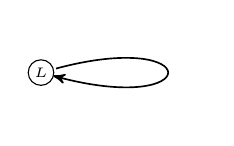
\begin{tikzpicture}[scale = 4]
\tikzstyle{VertexStyle}=[shape = circle,	
								 minimum size = 8pt,
								 inner sep = 1.2pt,
                         draw]

\Vertex[x = 0.0, y = 0.0, L = \tiny {$L$}]{v0}
\Edge[style = {loop right, post}](v0)(v0)
\end{tikzpicture}

\caption{The Liar graph.}
\end{figure}
%%


%% yablo graph %%
\begin{figure}[h]
\centering
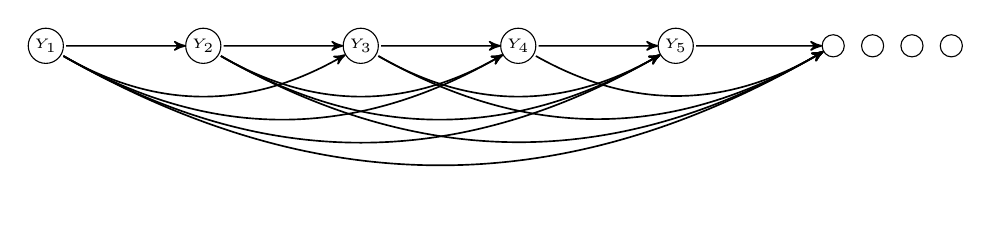
\begin{tikzpicture}[scale = 10]
\tikzstyle{VertexStyle}=[shape = circle,	
								 minimum size = 8 pt,
								 inner sep = 1.2pt,
                         draw]
\Vertex[x = 0.0, y = 0.5, L = \tiny {$Y_1$}]{v0}
\Vertex[x = 0.2, y = 0.5, L = \tiny {$Y_2$}]{v1}
\Vertex[x = 0.4, y = 0.5, L = \tiny {$Y_3$}]{v2}
\Vertex[x = 0.6, y = 0.5, L = \tiny {$Y_4$}]{v3}
\Vertex[x = 0.8, y = 0.5, L = \tiny {$Y_5$}]{v4}
\Vertex[style = {draw = none}, x = 1.0, y = 0.5, L = \tiny {}]{v5}
\Vertex[style = {minimum size = 1 pt}, x = 1.05, y = 0.5, L = \tiny {}]{v6}
\Vertex[style = {minimum size = 1 pt}, x = 1.1, y = 0.5, L = \tiny {}]{v7}
\Vertex[style = {minimum size = 1 pt}, x = 1.15, y = 0.5, L = \tiny {}]{v8}
\Edge[style = {post}](v0)(v1)
\Edge[style = {bend right, post}](v0)(v2)
\Edge[style = {bend right, post}](v0)(v3)
\Edge[style = {bend right, post}](v0)(v4)
\Edge[style = {bend right, post}](v0)(v5)
\Edge[style = {post}](v1)(v2)
\Edge[style = {bend right, post}](v1)(v3)
\Edge[style = {bend right, post}](v1)(v4)
\Edge[style = {bend right, post}](v1)(v5)
\Edge[style = {post}](v2)(v3)
\Edge[style = {bend right, post}](v2)(v4)
\Edge[style = {bend right, post}](v2)(v5)
\Edge[style = {post}](v3)(v4)
\Edge[style = {bend right, post}](v3)(v5)
\Edge[style = {post}](v4)(v5)
\end{tikzpicture}
\caption{The Yablo graph.}
\end{figure}
%%

\begin{defn}
We call a directed graph $G$ \emph{dangerous} if there exists a paradoxical pair $(\S, d)$ such that $G$ is isomorphic to $\G_{\S, d}$.
\end{defn}

\begin{defn}
We call a directed graph $G$ \emph{precarious} if there exists a hypodoxical pair $(\S, d)$ such that $G$ is isomorphic to $\G_{\S, d}$.
\end{defn}

\begin{defn}
Let $G$ be a directed graph.  We write $N^{+}_G(v)$ for the set of neighbors of $v$ in $G$ to which $v$ has an edge and $N^{-}_G(v)$ for the set of neighbors of $v$ in $G$ from which $v$ has an edge.
\end{defn}

%% neighbors %%
\begin{figure}[h]
\centering
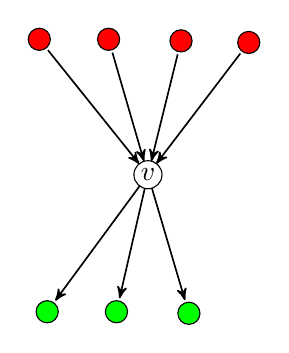
\begin{tikzpicture}[scale = 10]
\tikzstyle{VertexStyle}=[shape = circle,	
								 minimum size = 8pt,
								 inner sep = 1.2pt,
                         draw]
\Vertex[style = {fill = green}, x = 0.351999998092651, y = 0.396000027656555, L = \tiny {}]{v0}
\Vertex[style = {fill = green}, x = 0.439999967813492, y = 0.396000027656555, L = \tiny {}]{v1}
\Vertex[style = {fill = green}, x = 0.531999945640564, y = 0.393999993801117, L = \tiny {}]{v2}
\Vertex[x = 0.479999989271164, y = 0.569999992847443, L = {$v$}]{v3}
\Vertex[style = {fill = red}, x = 0.342000007629395, y = 0.742000013589859, L = \tiny {}]{v4}
\Vertex[style = {fill = red}, x = 0.429999977350235, y = 0.741999983787537, L = \tiny {}]{v5}
\Vertex[style = {fill = red}, x = 0.521999955177307, y = 0.739999979734421, L = \tiny {}]{v6}
\Vertex[style = {fill = red}, x = 0.607999980449677, y = 0.738000005483627, L = \tiny {}]{v7}
\Edge[style = {pre}](v0)(v3)
\Edge[style = {pre}](v1)(v3)
\Edge[style = {pre}](v2)(v3)
\Edge[style = {post}](v4)(v3)
\Edge[style = {post}](v5)(v3)
\Edge[style = {post}](v6)(v3)
\Edge[style = {post}](v7)(v3)
\end{tikzpicture}
\caption{$N^{-}_G(v)$ in red and $N^{+}_G(v)$ in green.}
\end{figure}
%%

\section{Danger Preserving Operations}
\label{sec3}

We will need some basic lemmas about (weakly) dangerous graphs.

\subsection{Subgraphs}

\begin{lem}\label{SubgraphDangerLemma}
Let $G$ be a directed graph.  Then $G$ is dangerous (precarious) if and only if some subgraph of $G$ is dangerous (precarious).
\end{lem}
\begin{proof}
Since $G$ is a subgraph of itself, the forward implication is immediate.  For the reverse implication, let $H$ be a subgraph of $G$ that is dangerous (precarious).  View $V(H)$ as a set of sentence names and let $d$ be a denotation assignment on $V(H)$ such that $(V(H), d)$ is paradoxical (hypodoxical) and
$H = \G_{V(H), d}$. \newline 

We construct a denotation assignment $d'$ on $V(G)$ by employing junk conjunctions $J_x = \bot \wedge \bigwedge_{y \in N^{+}_G(x)} y$, for each $x \in V(G)$. The denotation assignment $d'$ assigns to $x$ a sentence containing its junk conjunction -- this gets the referencing right, but the junk sentences must be added in such a way that they have no impact on the acceptability of truth-value assignments. For $x \in V(G)$, let

\[d'(x) = \begin{cases}
d(x) \vee J_x & \text{if } x \in V(H) \\
J_x & \text{if } x \not \in V(H)
\end{cases}.\]

Then, by construction, $G = \G_{V(G), d'}$ and $(V(G), d')$ is paradoxical (hypodoxical).  Hence $G$ is dangerous (precarious).
\end{proof}

Add diagram?

\subsection{Smoothing and Subdividing}

Given a pair $(\S, d)$, intuitively we can ``simplify'' it to a pair $(\S', d')$ by picking some $\alpha \in \S$, replacing every occurance of $\alpha$ with $d(\alpha)$ and then removing $\alpha$ from $\S$.  Doing so gives rise to a danger preserving operation on graphs.  

\begin{lem}\label{SubstitutionLemma}
Let $\S$ be a set and let $\psi \in \S^+$.  Let $v$ be a truth-value assignment on $\S$.  Let $\left\{ (\alpha_i, \gamma_i)\right\}_{i \in I} \subseteq \S \times \S^+$ such that the $\alpha_i$ are pairwise distinct. If $v(\alpha_i) = \llbracket \gamma_i \rrbracket(v)$ for each $i \in I$, then

\[\left\llbracket \psi\left[\alpha_i \Rightarrow \gamma_i \mid i \in I\right]\right\rrbracket(v) = \llbracket \psi \rrbracket(v).\] 
\end{lem}
\begin{proof}
This is immediate from the definition of the semantics.
\end{proof}

Consider a pair $(\S, d)$ and $\alpha \in \S$ such that $\alpha$ does not occur as a constituent of $d(\alpha)$. Let $\S' = \S - \{\alpha\}$ and for $\beta \in \S'$ let $d'(\beta) = d(\beta)\left[\alpha \Rightarrow d(\alpha)\right]$.  Then $d'$ is a denotation assignment on $\S'$. Given a truth assignment $v$ on $\S$, let $v'$ be $v$ restricted to $S'$.  Then, by Lemma \ref{SubstitutionLemma}, $v$ is acceptable on $\S$ relative to $d$ if and only if $v'$ is acceptable on $\S'$ relative to $d'$.  Thus the following ``smoothing'' operation leaves dangerous graphs dangerous and precarious graphs precarious.

\begin{defn}
Let $G$ be a directed graph.  Let $y \in V(G)$ such that $yy \not \in E(G)$.  The \emph{smoothing} of $G$ at $y$ is the graph $H$ with $V(H) = V(G) - y$ and
$E(H) = E(G - y) \cup \left\{ab \mid a \in N^-(y), b \in N^+(y)\right\}$.
\end{defn}

%% smoothing %%
\tikzstyle{VertexStyle}=[shape = circle,	
  								 minimum size = 1pt,
								 inner sep = 1.2pt,
								 draw]

\begin{figure}[h]
\centering
\subfloat[] {
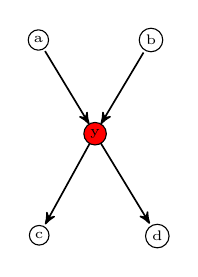
\begin{tikzpicture}[scale = 10]
\tikzstyle{VertexStyle}=[shape = circle,	
								 minimum size = 1pt,
								 inner sep = 1.2pt,
                         draw]
\Vertex[x = 0.219333365559578, y = 0.701000034809113, L = \tiny {c}]{v0}
\Vertex[x = 0.369333326816559, y = 0.699999988079071, L = \tiny {d}]{v1}
\Vertex[style = {fill=red}, x = 0.290333330631256, y = 0.830000028014183, L = \tiny {y}]{v2}
\Vertex[x = 0.218333393335342, y = 0.949000023305416, L = \tiny {a}]{v3}
\Vertex[x = 0.361333340406418, y = 0.948999986052513, L = \tiny {b}]{v4}
\Edge[style = {post}](v3)(v2)
\Edge[style = {post}](v4)(v2)
\Edge[style = {pre}](v0)(v2)
\Edge[style = {pre}](v1)(v2)
\end{tikzpicture}
}
\subfloat[] {
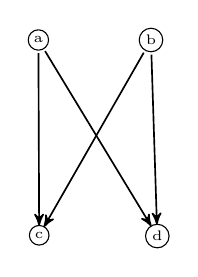
\begin{tikzpicture}[scale = 10]
\tikzstyle{VertexStyle}=[shape = circle,	
								 minimum size = 1pt,
								 inner sep = 1.2pt,
                         draw]
\Vertex[x = 0.219333365559578, y = 0.701000034809113, L = \tiny {c}]{v0}
\Vertex[x = 0.369333326816559, y = 0.699999988079071, L = \tiny {d}]{v1}
\Vertex[x = 0.218333393335342, y = 0.949000023305416, L = \tiny {a}]{v2}
\Vertex[x = 0.361333340406418, y = 0.948999986052513, L = \tiny {b}]{v3}
\Edge[style = {post}](v2)(v0)
\Edge[style = {post}](v3)(v0)
\Edge[style = {post}](v2)(v1)
\Edge[style = {post}](v3)(v1)
\end{tikzpicture}
}
\caption{A graph and its smoothing at $y$.}
\end{figure}
%%

The reverse operation of introducing a new name doesn't behave nicely in general, but it does in a few interesting special cases. One is that of a subdivision.

\begin{defn}
Let $G$ be a directed graph.  A \emph{subdivision} of $G$ is a graph formed by replacing each edge $xy$ of $G$ with a path $p_{xy}$ from $x$ to $y$.  Note that we allow $p_{xy}$ to be length $1$; that is, $p_{xy} = xy$.
\end{defn}

% subdivision %

\begin{figure}[h]
\centering
\subfloat[] {
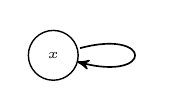
\begin{tikzpicture}[scale = 2]

\Vertex[x = 0.0, y = 0.0, L = \tiny {$x$}]{v0}
\Edge[style = {loop right, post}](v0)(v0)
\end{tikzpicture}
}
\subfloat[] {
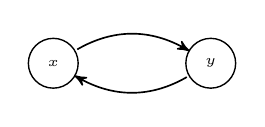
\begin{tikzpicture}[scale = 2]
\Vertex[x = 0.0, y = 0.0, L = \tiny {$x$}]{v0}
\Vertex[style = {fill = green}, x = 1.0, y = 0.0, L = \tiny {$y$}]{v1}
\Edge[style = {bend left, post}](v0)(v1)
\Edge[style = {bend left, post}](v1)(v0)
\end{tikzpicture}
}
\subfloat[] {
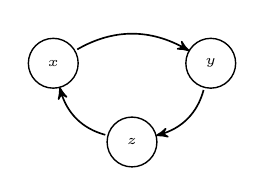
\begin{tikzpicture}[scale = 2]
\Vertex[x = 0.0, y = 0.0, L = \tiny {$x$}]{v0}
\Vertex[x = 1.0, y = 0.0, L = \tiny {$y$}]{v1}
\Vertex[style = {fill = green}, x = 0.5, y = -0.5, L = \tiny {$z$}]{v2}
\Edge[style = {bend left, post}](v0)(v1)
\Edge[style = {bend left, post}](v1)(v2)
\Edge[style = {bend left, post}](v2)(v0)
\end{tikzpicture}
}
\caption{The Liar graph and two subdivisions.}
\end{figure}
%%

\begin{lem}\label{SubdivisionLemma}
A subdivision of a directed graph $G$ is dangerous if and only if $G$ is.
\end{lem}
\begin{proof}
First, assume $G$ is dangerous and let $d$ be a denotation assignment on $V(G)$ such that $G = \G_{V(G), d}$ and $(V(G), d)$ is paradoxical.  Let $H$ be the subdivision of $G$ where each edge $xy \in E(G)$ is replaced with the path $p_{xy}$ from $x$ to $y$.  Say the vertices of $p_{xy}$ in order are $x = z_{xy}^1, z_{xy}^2, \ldots, z_{xy}^{k_{xy}} = y$.  Define a denotation assignment $d'$ on $V(H)$ by

\[d'(w) = \begin{cases}
d(w)[y \Rightarrow z_{wy}^2 \mid wy \in E(G)] & \text{if } w \in V(G) \\
z_{xy}^{j+1} & \text{if } w = z_{xy}^j \text{ for } xy \in E(G), j \geq 2 \\
\end{cases}.\]

By construction we have $H = \G_{V(H), d'}$.  Now we will show that $H$ is paradoxical with this denotation assignment.  Assume not and let $v'$ be an acceptable truth assignment on $V(H)$ with respect to $d'$ and let $v$ be $v'$ restricted to $V(G)$. Then for each $xy \in E(G)$ and $2 \leq j < k_{xy}$ we have $\llbracket d'(z_{xy}^j) \rrbracket(v') = \llbracket z_{xy}^{j + 1} \rrbracket(v')$.  Hence $v'(z_{xy}^2) = \llbracket d'(z_{xy}^2) \rrbracket(v') = \llbracket d'(y) \rrbracket(v') = v'(y)$ since $v'$ is acceptable.  Thus for $w \in V(G)$, by Lemma \ref{SubstitutionLemma}, we have $v(w) = v'(w) = \llbracket d'(w) \rrbracket(v') = \llbracket d(w)[y \Rightarrow z_{wy}^2 \mid wy \in E(G)] \rrbracket(v') = \llbracket d(w) \rrbracket(v') = \llbracket d(w) \rrbracket(v)$.  Whence $v$ is acceptable on $V(G)$ with respect to $d$.  This contradicts the fact that $G$ is dangerous.\newline

The other direction is very similar, basically we smooth at all of the subdivision vertices.  We omit the proof to avoid unnecessary tedium.
\end{proof}

We can use this to prove that being dangerous is a topological property of directed graphs.

\begin{defn}
Two directed graphs $G$ and $H$ are \emph{homeomorphic} if some subdivision of $G$ is isomorphic to some subdivision of $H$.
\end{defn}

\begin{lem}
If $G$ and $H$ are homeomorphic directed graphs, then $G$ is dangerous if and only if $H$ is dangerous.
\end{lem}
\begin{proof}
Assume $G$ and $H$ are homeomorphic directed graphs and let $G'$ and $H'$ be subdivisions of $G$ and $H$ respectively such that $G'$ is isomorphic to $H'$. The lemma follows by applying Lemma \ref{SubdivisionLemma} to $G$ and $G'$ and to $H$ and $H'$.
\end{proof}

\begin{comment}
\subsection{Partitioning}

if you can divide your graph into two so that both are not dangerous and edges go only one way between them then the whole thing is not dangerous.

\begin{lem}\label{PartitionLemma}
Let $G$ be a directed graph.  If $V(G)$ has a subset $A$ such that there are no edges from $A$ to $G - A$ and both $G[A]$ and $G - A$ are not dangerous, then $G$ is not dangerous.
\end{lem}
\begin{proof}
Assume $V(G)$ has a subset $A$ such that there are no edges from $A$ to $G - A$ and both $G[A]$ and $G - A$ are not dangerous.  Let $d$ be a denotation assignment on $V(G)$ such that $G = \G_{V(G), d}$.  Since $A$ has no edges to $G - A$ we see that $d$ restricted to $A$ is a denotation assignment on $A$, call it $d_A$.  Since $G[A]$ is not dangerous, we have an acceptable truth assignment $v_A$ on $A$ with respect to $d_A$.  Define $\kappa(0) = \bot$ and $\kappa(1) = \top$.  Now define a denotation assignment $d'$ on $G - A$ by letting $d'(x) = d(x)[\alpha \Rightarrow \kappa(v_A(\alpha)) \mid \alpha \in A]$.  Since $G - A$ is not dangerous, we have an acceptable truth assignment $v'$ on $V(G - A)$ with respect to $d'$.  By construction, the truth assignment $v$ defined by

\[v(x) = \begin{cases}
v_A(x) & \text{if } x \in A \\
v'(x) & \text{if } x \not \in A \\
\end{cases}\]

is acceptable on $V(G)$ with respect to $d$.  Since $d$ was arbitrary, $G$ is not dangerous.
\end{proof}
\end{comment}

\subsection{Unrolling}
Add unrolling.
Add picture.

\begin{comment}
\section{Removing Sinks}
\label{sec4}

Let $\S$ be a set of sentence names and $d$ a denotation assignment on $\S$.  If $\chi$ is a constant sentence, then its normal form references no other sentence.  So, if name $\alpha \in \S$ denotes $\chi$, then we can simplify $(\S, d)$ by replacing each occurance of $\alpha$ with $\chi$.  We will show that we can repeatedly apply this operation until no name denotes a constant sentence.

\begin{defn}
Let $G$ be a directed graph.  A vertex $v \in V(G)$ is called a \emph{sink} if $N^+_G(v)$ is empty and a \emph{source} if $N^-_G(v)$ is empty.
\end{defn}

%% sinks & sources %%
\begin{figure}[h]
\centering
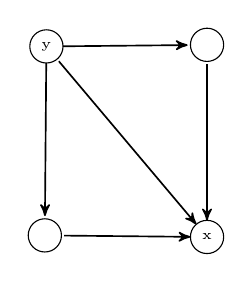
\begin{tikzpicture}[scale = 10]
\tikzstyle{VertexStyle}=[shape = circle,	
								 minimum size = 12pt,
								 inner sep = 1.2pt,
                         draw]
\Vertex[x = 0.605999946594238, y = 0.470000028610229, L = \tiny {x}]{v0}
\Vertex[x = 0.401999980211258, y = 0.712000012397766, L = \tiny {y}]{v1}
\Vertex[x = 0.606000065803528, y = 0.71399998664856, L = \tiny {}]{v2}
\Vertex[x = 0.400000005960464, y = 0.472000002861023, L = \tiny {}]{v3}
\Edge[style = {post}](v1)(v0)
\Edge[style = {pre}](v2)(v1)
\Edge[style = {post}](v2)(v0)
\Edge[style = {pre}](v3)(v1)
\Edge[style = {post}](v3)(v0)
\end{tikzpicture}
\caption{A graph with sink $x$ and source $y$.}
\end{figure}
%%

Note that a constant sentence (in normal form) corresponds to a sink in the graph.\newline

We will need to apply our substition infinitely many times.  To make this precise we need to index over some infinite ordinals.  For a set $X$, we write $|X|$ for the cardinal of $X$ which is the smallest ordinal which is equinumerous with $X$. 

\begin{defn}
Given a directed graph $G$, let $K(G)$ be the sinks of $G$ and $R(G) = G - K(G)$. Let $\R(G)$ be the induced subgraph of $G$ with vertex set $\bigcap_{n \leq 2^{|V(G)|}} V(R^n(G))$.
\end{defn}

\begin{lem}\label{NoSinksRemain}
If $G$ is a directed graph, then $\R(G)$ is sink-free.
\end{lem}
\begin{proof}
Assume (to reach a contradiction) that this is not the case and let $G$ be a graph for which $\R(G)$ contains a sink.  Let $O$ be the ordinal $2^{|V(G)|}$. For $l \leq O$, put $B_l = \bigcap_{n \leq l} V(R^n(G))$.  If for some $i < j \leq O$ we have $B_i = B_j$, then $B_i$ is sink-free and thus so is $\R(G)$.\newline

Thus we may assume that for each $i < O$ we have $b_i \in B_i$ such that $b_i \not \in B_j$ for any $i < j \leq O$.  In particular, $b_i \neq b_j$ for $i \neq j$.  Thus we may define $f: O \rightarrow V(G)$ by $f(i) = b_i$.  But this gives an injection from a set of cardinality $2^{|V(G)|}$ to a set of cardinality $|V(G)|$ which is a contradiction by Cantor's theorem.
\end{proof}

\begin{lem}\label{RemoveSinksPreservesDanger}
A directed graph $G$ is (weakly) dangerous if and only if $\R(G)$ is (weakly) dangerous.
\end{lem}
\begin{proof}
Put $H = \R(G)$. Since $H$ is a subgraph of $G$, the reverse direction follows from Lemma \ref{SubgraphDangerLemma}.\newline

For the forward direction, let $d$ be a denotation assignment on $V(G)$ such that $G = \G_{V(G), d}$ and $(V(G), d)$ is (weakly) paradoxical.\newline

The idea is to repeatedly simplify the sentences by substituting constant sentences in for their names.  Let $O$ be the ordinal $2^{|V(G)|}$. For 
$l \leq O$, put $B_l = \bigcap_{n \leq l} V(R^n(G))$ and $G_l = G[B_l]$. Note that $H = G_O$.  Put $f_0 = d$ and recursively define $d_l$ for $0 < l \leq O$ and $x \in V(G)$ by 

\[d_l(x) = d(x)\left[y \Rightarrow \zeta_{d_k(y)} \mid 0 \leq k < l, y \in K(G_{k})\right].\]

Let $d_H$ be $d_O$ restricted to $V(H)$.  Since all elements of $V(G) - V(H)$ were replaced with either $\top$ or $\bot$ in $d_O(x)$ for every $x \in V(G)$, we see that the image of $d_O$ is contained in $V(H)^+$. Thus $d_H$ is a denotation assignment on $V(H)$.  \newline

Let $v$ be a truth-value assignment on $V(H)$ with respect to $d_H$.  Consider the truth-value assignment $v'$ on $V(G)$ given by

\[v'(x) = \begin{cases}
v(x) & \text{if } x \in V(H)\\
c(d_O(x)) & \text{if } x \in V(G) - V(H)
\end{cases}.\]

Here $c(d_O(x))$ is the value of the constant sentence $d_O(x)$.  We claim that $v'$ is acceptable on $V(G)$ with respect to $d$ if and only if $v$ is acceptable on $V(H)$ with respect to $d_H$.  \newline

To see this, first assume that $v$ is acceptable on $V(H)$ with respect to $d_H$.  Then $v'(x) = v(x) = \llbracket d_H(x) \rrbracket(v) = \llbracket d_O(x) \rrbracket(v')$ for each $x \in V(H)$.  By Lemma \ref{SubstitutionLemma}, we have $\llbracket d_O(x) \rrbracket(v') = \llbracket d(x) \rrbracket(v')$ for $x \in V(G)$.  Hence $v'(x) = \llbracket d(x) \rrbracket (v')$ for $x \in V(H)$.  For $x \in V(G) - V(H)$ we have $v'(x) = c(d_O(x)) = \llbracket d_O(x) \rrbracket(v') = \llbracket d(x) \rrbracket(v')$ by Lemma \ref{SubstitutionLemma}. \newline

For the other direction, assume that $v'$ is acceptable on $V(G)$ with respect to $d$.  Then $v'(x) = \llbracket d(x) \rrbracket(v') = \llbracket d_O(x) \rrbracket(v')$ by Lemma \ref{SubstitutionLemma}.  Thus for $x \in V(H)$ we have $v(x) = v'(x) = \llbracket d_H(x) \rrbracket(v)$.  \newline

Therefore we have a bijection between the acceptable assignments on $V(G)$ with respect to $d$ and the acceptable acceptable assignments on $V(H)$ with respect to $d_H$.  In particular, $(V(H), d_H)$ is (weakly) paradoxical since $(V(G), d)$ is. Thus $H$ is (weakly) dangerous.
\end{proof}
\end{comment}

\section{Groundedness}
\label{sec5}

\begin{defn}
A \emph{ray} in a directed graph $G$ is a subgraph with vertex set $\{v_i\}_{i < \omega}$ and edge set $\{(v_i, v_{i + 1})\}_{i < \omega}$.
\end{defn}

%% ray %%
\begin{figure}[h]
\centering
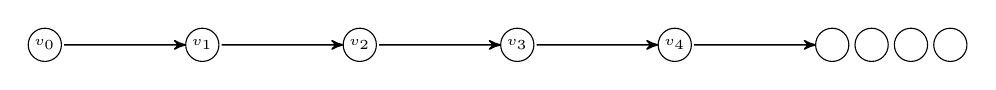
\begin{tikzpicture}[scale = 10]
\tikzstyle{VertexStyle}=[shape = circle,	
								 minimum size = 12 pt,
								 inner sep = 1.2pt,
                         draw]
\Vertex[x = 0.0, y = 0.5, L = \tiny {$v_0$}]{v0}
\Vertex[x = 0.2, y = 0.5, L = \tiny {$v_1$}]{v1}
\Vertex[x = 0.4, y = 0.5, L = \tiny {$v_2$}]{v2}
\Vertex[x = 0.6, y = 0.5, L = \tiny {$v_3$}]{v3}
\Vertex[x = 0.8, y = 0.5, L = \tiny {$v_4$}]{v4}
\Vertex[style = {draw = none}, x = 1.0, y = 0.5, L = \tiny {}]{v5}
\Vertex[style = {minimum size = 1 pt}, x = 1.05, y = 0.5, L = \tiny {}]{v6}
\Vertex[style = {minimum size = 1 pt}, x = 1.1, y = 0.5, L = \tiny {}]{v7}
\Vertex[style = {minimum size = 1 pt}, x = 1.15, y = 0.5, L = \tiny {}]{v8}
\Edge[style = {post}](v0)(v1)
\Edge[style = {post}](v1)(v2)
\Edge[style = {post}](v2)(v3)
\Edge[style = {post}](v3)(v4)
\Edge[style = {post}](v4)(v5)
\end{tikzpicture}
\caption{A ray.}
\end{figure}
%%

\begin{defn}
A directed graph $G$ is \emph{grounded} if it does not contain a ray or a directed cycle.  Otherwise $G$ is \emph{ungrounded}.
\end{defn}

Intuitively, if $G$ is grounded, then we can obtain an acceptable truth assignment for any denotation assignment on $V(G)$ by repeatedly substituting the values of constant sentences in for their names.  Since we don't make any arbitrary choices in this process, the constructed acceptable truth assignment should be unique.  To make performing this operation infinitely many times precise we will apply Zorn's lemma.  Later we will use a similar proof idea to prove a more general result.

\begin{zorn}
Every partially ordered set, in which every chain (i.e. totally ordered subset) has an upper bound, contains at least one maximal element.
\end{zorn}

\begin{defn}
Let $G$ be a directed graph.  We say that $A \subseteq V(G)$ is \emph{self-contained} in $G$ if there are no edges in $G$ directed from $A$ to $G - A$.  
\end{defn}

\begin{lem}\label{GroundedNotDangerous}
If a directed graph $G$ is grounded, then it is not dangerous and not precarious.
\end{lem}
\begin{proof}
Assume $G$ is grounded.  Let $d$ be a denotation assignment on $V(G)$ such that $G = \G_{V(G), d}$. We will show that there is a unique acceptable truth assignmement on $V(G)$ with respect to $d$.  Since $d$ was arbitrary, it follows that $G$ is not dangerous and not precarious.\newline

For $A \subseteq V(G)$ which is self-contained in $G$, let $d_A$ be $d$ restricted to $A$.  Then $d_A$ is a denotation assignment on $A$.  If $A$ has a unique acceptable truth assignment with respect to $d_A$, then we call this truth assignment $v_A$ and call the pair $(A, v_A)$ \emph{solved}.\newline

Let $X$ be the collection of all solved pairs.  Define a partial order $<$ on $X$ by $(A, v_A) < (B, v_B)$ if and only if $A \subsetneq B$ and $v_A$ is $v_B$ restricted to $A$.\newline

To apply Zorn's lemma to $(X, <)$, we need to show that $X \neq \emptyset$ and that every chain in  $(X, <)$ has an upper bound. Since $(\emptyset, v_\emptyset) \in X$ we see that $X \neq \emptyset$.  Now let $(A_1, v_{A_1}) < (A_2, v_{A_2}) < \cdots$ be an arbitrary chain in $(X, <)$.  Put $U = \bigcup_{i > 0} A_i$. Plainly, $U$ is self-contained in $G$. For $u \in U$, let $h(u)$ be the smallest $i > 0$ such that $u \in A_i$.  Now, for $u \in U$, let $v_U(u) = v_{A_{h(u)}}(u)$.  We claim that $(U, v_U)$ is an upper bound for the chain.  By definition $A_i \subseteq U$ and $v_{A_i}$ is $v_U$ restricted to $A_i$ for each $i > 0$.  It remains to be shown that $v_U$ is the unique acceptable truth assignment on $U$ with respect to $d_U$.  Assume $v_U$ is not acceptable and pick $u \in U$ with $h(u)$ minimal such that $v_U(u) \neq \llbracket d_U(u)\rrbracket(v_U)$.  Put $B = A_{h(u)}$. Then

\[v_B(u) = v_U(u) \neq \llbracket d_U(u)\rrbracket(v_U) = \llbracket d_B(u)\rrbracket(v_B) = v_B(u).\]

This is a contradiction.  Hence $v_U$ is acceptable.  To see that $v_U$ is unique, assume there is a different acceptable truth assignment on $U$ with respect to $d_U$, call it $v_O$.  Take $u \in U$ with $h(u)$ minimal such that $v_U(u) \neq v_O(u)$.  Again put $B = A_{h(u)}$.  Then $v_O$ restricted to $B$ is an acceptable truth assignment on $B$ with respect to $d_B$ which is different from $v_B$.  This is a contradiction.  Thus we conclude that $(U, v_U)$ is an upper bound for the chain.\newline

Applying Zorn's lemma gives us a solved pair $(M, v_M)$ which is maximal in $(X, <)$.  We will show that $M = V(G)$ and hence $v_M$ is the desired unique acceptable truth assignment on $V(G)$ with respect to $d$.  So assume $M \neq V(G)$.  Put $J = V(G) - M$. First assume that there is some $z \in J$ such that $T = M \cup \{z\}$ is self-contained.  Since $T$ is self-contained, $d(z)$ involves only elements of $M$.  Thus, letting $v_T(x) = v_M(x)$ for each $x \in M$ and $v_T(z) = d(z)[x \Rightarrow v_M(x) \mid x \in M]$ makes $v_T$ the unique acceptable truth assignment on $T$ with respect to $d_T$.  We conclude that $(T, v_T) \in X$ and $(M, v_M) < (T, v_T)$ contradicting the maximality of $(M, v_M)$.\newline

Thus we may assume that $N^+(z) \cap J \neq \emptyset$ for each $z \in J$.  Pick $z_0 \in J$.  For $k > 0$, let $z_k \in N^+(z_{k - 1}) \cap J$.  Since $G$ is acyclic, $z_0z_1z_2\cdots$ is a ray in $G$ contradicting the fact that $G$ is grounded.  Whence $M = V(G)$ and the proof is complete.
\end{proof}

\begin{lem}\label{DirectedCyclesMakeDanger}
If a directed graph $G$ contains a directed cycle, then it is both dangerous and precarious.
\end{lem}
\begin{proof}
By Lemma \ref{SubgraphDangerLemma}, we can assume that $G$ is a directed cycle.  Let $V(G) = \{v_1, \ldots, v_k\}$.  Let $d$ be a denotation assignment on $V(G)$ with $d(v_i) = \neg v_{i + 1}$ for $i < k$, $d(v_k) = \neg v_1$ if $k$ is odd and $d(v_k) = v_1$ if $k$ is even.  Then $G = \G_{V(G), d}$ and $(V(G), d)$ is paradoxical.  Hence $G$ is dangerous.  To see that $G$ is precarious, just consider the denotation assignment $d'$ on $V(G)$ with $d'(v_i) = v_{i + 1}$ for $i < k$ and $d(v_k) = v_1$.  Both the truth assignment setting all the $v_i$ to $1$ and the truth assiggment setting all the $v_i$ to $0$ are acceptable.
\end{proof}

\begin{thm}\label{PrecariousCharacterization}
A directed graph $G$ is precarious if and only if it is ungrounded.
\end{thm}
\begin{proof}
Lemma \ref{GroundedNotDangerous} gives the forward implication.  For the reverse implication, by Lemma \ref{SubgraphDangerLemma} and Lemma \ref{DirectedCyclesMakeDanger} we may assume that $G$ is a ray with vertex set $\{v_i\}_{i < \omega}$.  Let $d$ be a denotation assignment on $V(G)$ with $d(v_i) = v_{i+1}$.  Then $G = \G_{V(G), d}$ and $(V(G), d)$ is hypodoxical because we get two acceptable truth-value assignments by setting all the $v_i$ to $1$ or setting all the $v_i$ to $0$.
\end{proof}

\begin{cor}
If a directed graph is dangerous then it is precarious.
\end{cor}

In the finite case, it turns out that the dangerous and the precarious graphs coincide. Additionally, we have a complete characterization of the dangerous graphs.
\begin{cor}\label{FiniteCharacterization}
A finite directed graph is dangerous if and only if it contains a directed cycle.
\end{cor}

\begin{cor}\label{FiniteIsSubdividedLiar}
A finite directed graph is dangerous if and only if it contains a subdivision of the Liar graph.
\end{cor}

\begin{cor}
A finite directed graph is dangerous if and only if it is precarious.
\end{cor}

\begin{defn}
A \emph{homomorphism} from a directed graph $G$ to a directed graph $H$ is a function $f:V(G) \rightarrow V(H)$ such that if $xy \in E(G)$, then $f(x)f(y) \in E(H)$.   If $f$ is a bijection, and $f^{-1}: V(H) \rightarrow V(G)$ is a homomorphism, the we call $f$ an \emph{isomorphism}.  Additionally, we call the graph with vertex set $f(V(G))$ and edge set $\{f(x)f(y) \mid xy \in E(G)\}$ the \emph{homomorphic image} of $G$ under $f$.
\end{defn}

\begin{lem}
Let $G$ be a directed graph.  Then $G$ is precarious if and only if every homomorphic image of $G$ is precarious.
\end{lem}
\begin{proof}
Since $G$ is a homomorphic image of it self, the reverse implication is trivial.  To proved the forward implication, assume $G$ is precarious.  Then, by Theorem \ref{PrecariousCharacterization} $G$ contains a directed cycle or a ray.  Let $H$ be a homomorphic image of $G$ and let $f:V(G) \rightarrow V(H)$ be a homomorphism.  If there is a directed path between $x,y \in V(G)$, then we cannot have $f(x) = f(y)$, for otherwise $H$ would contain a directed cycle and hence be precarious.  In particular, $G$ cannot contain a directed cycle.  Thus $G$ contains a ray $\{v_i\}_{i < \omega}$.  If $f(v_i) = f(v_j)$ for $i \neq j$, then $H$ contains a directed cycle and we are done.  Otherwise $H$ contains a ray and we are done.
\end{proof}

\begin{conj}
Let $G$ be a directed graph.  Then $G$ is dangerous if and only if every homomorphic image of $G$ is dangerous.
\end{conj}

\section{Compactness Results}
\label{sec6}

Using compactness, we will show that graphs for which $N^+(v)$ is finite for every vertex $v$ are not dangerous. But, to apply compactness we need to have finite length sentences. The following generalization of Lemma \ref{LanguageIsCompleteSimple} gives us the control over the lengths of sentences that we need.

\begin{defn}
For $v \in \V_\S$ and $I \subseteq \S$, let
\[v^I = \left\{u \in  \V_\S \mid \forall_{\alpha \in \S - I} u(\alpha) = v(\alpha)\right\}.\]
\end{defn}

\begin{defn}
Let $g$ be a function from $\V_\S$ to $\{0, 1\}$.  We say that $g$ is \emph{independent of} $I \subseteq \S$ if $g$ is constant on $v^I$ for each $v \in \V_\S$.
\end{defn}

Note that every such function is independent of the empty set.

\begin{lem}\label{LanguageIsComplete}
For any function $g$ from $\V_\S$ to $\{0, 1\}$ and any $I \subseteq \S$ of which $g$ is independent we have a sentence $\zeta_{g, I} \in \S^+$ involving no sentence name from $I$ such that $\zeta_{g, I} = g$. Moreover, $\zeta_{g, I}$ has finite length if $\S - I$ is finite.
\end{lem}

\begin{proof}
Let $g$ be a function from $\V_\S$ to  $\{0, 1\}$.  First, if $g$ is a constant function, put $\zeta_{g, I} = \top$ if $g$ maps everything to $1$ and $\zeta_{g, I} = \bot$ if $g$ maps everything to $0$.\newline

Otherwise $\S - I$ has at least one element and we proceed as follows.  Let $B = \{v \in \V_\S \mid \forall_{\alpha \in I} v(\alpha) = 0\}$. Note that $g$ is completely determined by its values on the elements of $B$. \newline

For $v \in \V_\S$ and $\alpha \in \S$, let 

\[P(v, \alpha) = \begin{cases}
\alpha & \text{if } v(\alpha) = 1 \\
\neg \alpha & \text{if } v(\alpha) = 0
\end{cases}.\]

Let $C = \{v \in B \mid g(v) = 1 \}$. For $v \in C$, define

\[\chi_v = \bigwedge_{\alpha \in \S - I} P(v, \alpha).\] 

Note that $\chi_v(r) = g(r)$ if $r = v$ and $\chi_v(r) = 0$ if $r \neq v$. Let $\zeta_{g, I}$ be the sentence
\[\bigvee_{v \in C} \chi_v.\]

Then, for any $r \in \V_\S$, we have 

\[\llbracket \zeta_{g, I} \rrbracket(r) = \left\llbracket\bigvee_{v \in C} \chi_v \right\rrbracket(r) = \bigvee_{v \in C} \llbracket \chi_v \rrbracket(r) = \llbracket \chi_r \rrbracket(r) = g(r).\]

Hence $\zeta_{g, I} = g$.  Now the length of  $\zeta_{g, I}$ is at most $|C||\S - I| \leq |B||\S - I| \leq 2^{|\S - I|}|\S - I|$. Thus $\zeta_{g, I}$ has finite length if  $\S - I$ is finite. 
\end{proof}

\begin{lem}\label{LocalFinite}
Let $G$ be a directed graph such that $|N^{+}_G(v)|$ is finite for every $v \in V(G)$.  If $G$ is dangerous then some finite subraph of $G$ is dangerous.
\end{lem}
\begin{proof}
Assume that no finite subgraph of $G$ is dangerous and let $d$ be a denotation assignment on $V(G)$ such that $G = \G_{V(G), d}$.  For each $v \in V(G)$, put $I_v = V(G) - N^+_G(v)$. Construct a first order language $\fancy{L}$ as follows.  The constants of $\L$ are the vertices of $G$ together with $\top$ and $\bot$.  The axioms are the following.

\begin{itemize}
\item $\top \neq \bot$
\item $x = \top \vee x = \bot$ for each $x \in V(G)$,
\item $x = \zeta_{\llbracket d(x) \rrbracket, I_x}$ for each $x \in V(G)$.
\end{itemize}

By Lemma \ref{LanguageIsComplete} each of the sentences is of finite length.  Note that a model of the language is an acceptable truth assignment on $V(G)$ relative to $d$.  Since no finite subgraph of $G$ is dangerous, every finite subset of the axioms has a model.  Thus, by compactness, the whole language has a model and hence $(V(G), d)$ is not paradoxical.  Since $d$ was arbitrary, we conclude that $G$ is not dangerous.
\end{proof}

\begin{cor}\label{AtLeastOneInfinite}
Any directed acyclic graph $G$ such that $|N^{+}_G(v)|$ is finite for every $v \in V(G)$ is not dangerous.
\end{cor}
\begin{proof}
Combine Corollary \ref{FiniteCharacterization} and Lemma \ref{LocalFinite}.
\end{proof}


No we show that if $G$ is an acyclic directed graph then its vertices can be ordered left to right such that edges only go to the right.  

\begin{defn}
Let $G$ be a directed graph.  A vertex $v \in V(G)$ is called a \emph{sink} if $N^+_G(v)$ is empty and a \emph{source} if $N^-_G(v)$ is empty.
\end{defn}

%% sinks & sources %%
\begin{figure}[h]
\centering
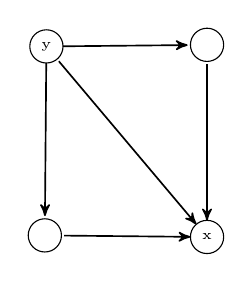
\begin{tikzpicture}[scale = 10]
\tikzstyle{VertexStyle}=[shape = circle,	
								 minimum size = 12pt,
								 inner sep = 1.2pt,
                         draw]
\Vertex[x = 0.605999946594238, y = 0.470000028610229, L = \tiny {x}]{v0}
\Vertex[x = 0.401999980211258, y = 0.712000012397766, L = \tiny {y}]{v1}
\Vertex[x = 0.606000065803528, y = 0.71399998664856, L = \tiny {}]{v2}
\Vertex[x = 0.400000005960464, y = 0.472000002861023, L = \tiny {}]{v3}
\Edge[style = {post}](v1)(v0)
\Edge[style = {pre}](v2)(v1)
\Edge[style = {post}](v2)(v0)
\Edge[style = {pre}](v3)(v1)
\Edge[style = {post}](v3)(v0)
\end{tikzpicture}
\caption{A graph with sink $x$ and source $y$.}
\end{figure}
%%

\begin{defn}
Let $G$ be a directed graph.  A \emph{topological sort} on $G$ is a total ordering $<$ of $V(G)$ such that if $(a,b) \in E(G)$, then $a < b$.
\end{defn}

We prove the following easy lemma for completeness.
\begin{lem}
If $G$ is a finite directed acyclic graph, then $G$ has a topological sort.
\end{lem}
\begin{proof}
Assume (to reach a contradiction) that the lemma is false and let $G$ be a counterexample with the minimum number of vertices.  Since $G$ is finite it has a source $v$.  By minimality $G - v$ has a topological sort $\{v_1, \ldots, v_r\}$.  But then $\{v, v_1, \ldots, v_r\}$ is a topological sort of $G$. This is a contradiction.
\end{proof}

\begin{lem}\label{TopSortExists}
Let $G$ be an directed acyclic graph. Then $G$ has a topological sort.
\end{lem}
\begin{proof}
We construct a first order language $\fancy{L}$ and apply the compactness theorem.  Let the elements of $V(G)$ be the constants of $\fancy{L}$ and let $R$ be $\fancy{L}$'s only relation symbol.  Define the axioms of $\fancy{L}$ as follows.

\begin{itemize}
\item $\neg (a = b)$ for all distinct $a,b \in V(G)$,
\item $aRb$ for all $(a,b) \in E(G)$,
\item $aRb \rightarrow \neg (bRa)$ for all $a,b \in V(G)$,
\item $aRb \vee bRa \vee a = b$ for all $a,b \in V(G)$,
\item $(aRb \wedge bRc) \rightarrow aRc$ for all $a,b,c \in V(G)$.
\end{itemize}

Let $A$ be a finite subset of the axioms.  Let $C$ be the set of all constants appearing in some axiom of $A$.  Create $A'$ from $A$ by adding in all axioms involving only the elements of $C$.  Then $A'$ is still finite and if $A'$ has a model, so does $A$.  Put $H = G[C]$.  Since $H$ is finite and acyclic it has a topological sort $<$.  Letting $<$ be the interpretation of $R$ gives a model of $A'$ and hence $A$.\newline

Thus, by the compactness theorem, the entire set of axioms has a model.  The interpretation of $R$ in this model is the desired topological sort.
\end{proof}

\begin{lem}\label{GeneralZorn}
Let $G$ be a directed graph. If for every induced subgraph $H$ of $G$ there exists $\emptyset \neq C \subseteq V(H)$ which is self-contained in $H$ such that $G[C]$ is not dangerous, then $G$ is not dangerous.
\end{lem}
\begin{proof}
Assume that for every induced subgraph $H$ of $G$ there exists $\emptyset \neq C \subseteq V(H)$ which is self-contained in $H$ such that $G[C]$ is not dangerous.  Let $d$ be a denotation assignment on $V(G)$ such that $G = \G_{V(G), d}$. We will show that there is an acceptable truth assignmement on $V(G)$ with respect to $d$.  Since $d$ was arbitrary, it follows that $G$ is not dangerous.\newline

For $A \subseteq V(G)$ which is self-contained in $G$, let $d_A$ be $d$ restricted to $A$.  Then $d_A$ is a denotation assignment on $A$.  If $A$ has an  acceptable truth assignment with respect to $d_A$, then we pick an acceptable truth assignment $v_A$ and call the pair $(A, v_A)$ \emph{solved}.\newline

Let $X$ be the collection of all solved pairs.  Define a partial order $<$ on $X$ by $(A, v_A) < (B, v_B)$ if and only if $A \subsetneq B$ and $v_A$ is $v_B$ restricted to $A$.\newline

To apply Zorn's lemma to $(X, <)$, we need to show that $X \neq \emptyset$ and that every chain in  $(X, <)$ has an upper bound. Since $(\emptyset, v_\emptyset) \in X$ we see that $X \neq \emptyset$.  Now let $(A_1, v_{A_1}) < (A_2, v_{A_2}) < \cdots$ be an arbitrary chain in $(X, <)$.  Put $U = \bigcup_{i > 0} A_i$. Plainly, $U$ is self-contained in $G$. For $u \in U$, let $h(u)$ be the smallest $i > 0$ such that $u \in A_i$.  Now, for $u \in U$, let $v_U(u) = v_{A_{h(u)}}(u)$.  We claim that $(U, v_U)$ is an upper bound for the chain.  By definition $A_i \subseteq U$ and $v_{A_i}$ is $v_U$ restricted to $A_i$ for each $i > 0$.  It remains to be shown that $v_U$ is an acceptable truth assignment on $U$ with respect to $d_U$.  Assume $v_U$ is not acceptable and pick $u \in U$ with $h(u)$ minimal such that $v_U(u) \neq \llbracket d_U(u)\rrbracket(v_U)$.  Put $B = A_{h(u)}$. Then

\[v_B(u) = v_U(u) \neq \llbracket d_U(u)\rrbracket(v_U) = \llbracket d_B(u)\rrbracket(v_B) = v_B(u).\]

This is a contradiction.  Hence $v_U$ is acceptable.  Thus we conclude that $(U, v_U)$ is an upper bound for the chain.\newline

Applying Zorn's lemma gives us a solved pair $(M, v_M)$ which is maximal in $(X, <)$.  We will show that $M = V(G)$ and hence $v_M$ is the desired acceptable truth assignment on $V(G)$ with respect to $d$.  So assume $M \neq V(G)$.  Put $H = G - M$.  By assumption, we have $\emptyset \neq C \subseteq V(H)$ which is self-contained in $H$ such that $G[C]$ is not dangerous.  Put $B = M \cup C$.  Note that $B$ is self-contained.  Since $C$ is not dangerous, we can extend $v_M$ to an acceptable truth assignment $v_B$ on $B$ with respect to $d_B$.  But then $(B, v_B) \in X$ and $(B, v_B) > (M, v_M)$ contradicting the maximality of $(M, v_M)$. Hence $M = V(G)$ and the proof is complete.
\end{proof}


A good way to get self-contained sets in an acyclic graph is to topological sort the graph and take all vertices ``to the right'' of a given vertex.  To make this precise we introduce the concept of a tail.

\begin{defn}
Let $G$ be a directed acyclic graph and let $<$ be a topological sort on $G$.  For $z \in V(G)$, the $z$-tail of $G$ (with respect to $<$) is the subgraph induced on $\{x \in V(G) \mid x > z\}$.  An induced subgraph of $G$ that is a $z$-tail for some $z \in V(G)$ is called a \emph{tail} of $G$.
\end{defn}

\begin{lem}\label{TailLemma}
Let $G$ be a directed acyclic graph and let $<$ be a topological sort on $G$.  If every induced subgraph of $G$ has a tail which is not dangerous, then $G$ is not dangerous.
\end{lem}
\begin{proof}
Let $H$ be an arbitrary induced subgraph of $G$.  We need to show that there exists $\emptyset \neq A \subseteq V(H)$ which is self-contained in $H$ such that $G[A]$ is not dangerous.  Pick $z \in V(H)$ such that the $z$-tail of $H$ is not dangerous.  Let $T_z$ be the $z$-tail of $H$.  Note that $T_z$ is self-contained.  Thus, if $T_z$ is non-empty, then we are done.  Hence we may assume that $T_z$ is empty.  But then $x \leq z$ for every $x \in V(H)$.  Hence $z$ is a sink in H and in particular, $\{z\}$ is a non-empty, self-contained set which induces a non-dangerous graph.  This completes the proof.
\end{proof}

\begin{cor}\label{InfinitelyManyInfinite}
If $G$ is a dangerous directed acyclic graph, then $|N^{+}_G(v)|$ is infinite for infinitely many $v \in V(G)$.
\end{cor}
\begin{proof}
Let $G$ be a directed acyclic graph $G$ such that $|N^{+}_G(v)|$ is infinite for only finitely many $v \in V(G)$.  By Lemma \ref{TopSortExists} $G$ has a topological sort $<$.  Let $H$ be an arbitrary induced subgraph of $G$. Since there are only finitely many $v \in V(H)$ with $|N^{+}_G(v)|$ infinite, there is a largest (under the order $<$) such vertex $z_H$.  Then the $z_H$-tail of $H$ has no vertices with infinite out degree and hence is not dangerous by Lemma \ref{LocalFinite}.  Thus every induced subgraph of $G$ has a non-dangerous tail.  Applying Lemma \ref{TailLemma} finishes the proof.
\end{proof}

\section{Interrelatedness}
Let $\S = \{A_1, A_2, \ldots\}$ and $d(A_i) = \neg A_{i+1}$.  Then the reference graph of the pair $(\S, d)$ is the ray and we know that this is precarious but not dangerous from above.  Intuitively, in the reference graph we have an edge from $A_1$ to $A_2$ because $d(A_1)$ is ``a function of'' of $A_2$ (we will see in the Examples section that defining a graph based on ``dependence'' turns out to be useless in general). In this case, fixing the value of $A_2$ determines what the value of $A_1$ must be.  But it is also true that fixing the value of $A_1$ determines what the value of $A_2$ must be.  Looking at it this way, we would want to see an edges going both directions.  We can capture these intuitive ideas by considering necessary and sufficient conditions for danger on the underlying undirected graph of a directed graph $G$.

\begin{defn}
Let $G$ be a directed graph.  The \emph{underlying undirected graph} of $G$ is the graph $\fancy{U}(G)$ with vertex set $V(G)$ and an edge between $x, y \in V(G)$ if and only if $xy \in E(G)$ or $yx \in E(G)$.  We also call $G$ an \emph{orientation} of $\fancy{U}(G)$.
\end{defn}

It turns out that we can completely classify the undirected graphs which have dangerous orientations -- they are precisely the acyclic ones.  

\begin{thm}
A graph has a dangerous orientation if and only if it contains a cycle.
\end{thm}
\begin{proof}
The reverse direction is easy, since if $F$ is a graph that contains a cycle we may orient the edges of the cycle clockwise and the other edges arbitrarily and conclude that the orientation is dangerous using Lemma \ref{DirectedCyclesMakeDanger}.\newline

For the forward direction, assume $G$ is a directed graph such that $\fancy{U}(G)$ is acyclic.  Let $d$ be a denotation assignment on $V(G)$ such that $G = \G_{V(G), d}$.
\end{proof}

\section{The global function}
\label{sec7}

\begin{defn}
Let $\S$ be a set of sentence names and $d$ a denotation assignment on $\S$. The \emph{global function} $\F_{\S, d} :\V_\S \rightarrow \V_\S$ is given by $\F_{\S, d}(v)(\alpha) = \llbracket d(\alpha) \rrbracket(v)$.  Going the other direction, any function $f: \V_\S \rightarrow \V_\S$ gives rise to a denotation assignment $d_f$ on $S$ as follows.  For each $\alpha \in \S$, let $f_{\alpha}: \V_\S \rightarrow \{0, 1\}$ be given by $f_{\alpha}(v) = f(v)(\alpha)$.  Then put $d_f(\alpha) = \zeta_{f_{\alpha}}$ for each $\alpha \in \S$.  Note that these constructions are inverses of each other, that is $\F_{\S, d_f} = f$ and $d_{\F_{\S, d}} = d$.
\end{defn}

\begin{lem}
Let $\S$ be a set of sentence names and $d$ a denotation assignment on $\S$.  The pair $(\S, d)$ is paradoxical (hypodoxical) if and only if $\F_{\S, d}$ has zero (more than one) fixed point.
\end{lem}
\begin{proof}
Just note that $v \in \V_\S$ is a fixed point of $\F_{\S, d}$ if and only if $v(\alpha) = \F_{\S, d}(v)(\alpha) = \llbracket d(\alpha) \rrbracket(v)$ if and only if $v$ is a acceptable truth assignment on $\S$ with respect to $d$.
\end{proof}

This formulation is quite useful for constructing examples.  Let $\S$ be the natural numbers $\mathbb{N}$.  Then any function from the unit interval to itself without a fixed point will give rise to a paradoxical denotation assignment on $\S$.\newline

(the one below actually is one constructed this way)

\section{Examples}

\subsection{Paradox on irrationals}
[Talk about how it seems natural to define ``dependence'', but it fails in general, the following gives an example of a dangerous graph whose dependence graph has no edges.  Talk about dependence and reference coming apart in the general case as opposed to Cook's case.]\newline

Let $\S = \{S_k\}_{k < \omega}$ be a set of sentence names.   For each $k < \omega$ define a function $h_k:\V_\S \rightarrow [0,1]$ by $h_k(v) = 0.v(S_{k+1})v(S_{k+2})v(S_{k+3})\ldots$.  Now for each $k < \omega$ define a function $g_k:\V_\S \rightarrow \fancy{T}$ as follows. For $v \in \V_\S$, let 

\[g_k(s) = \begin{cases}
1 & \text{if } h_k(s) \in \mathbb{Q} \text{ and the $k$-th digit of the reduced binary form of $\frac{\sqrt{2}}{2}$ is $1$,}\\
0 & \text{otherwise}
\end{cases}.\]

Now by Lemma \ref{LanguageIsComplete}, for each $k < \omega$ we have $\gamma_k \in \S$ such that $\gamma_k(v) = g_k(v)$ for each $v \in \V_\S$.  Let $d$ be a denotation assignment on $\S$ such that $d(S_k) = \gamma_k$.\newline

We claim that $(\S, d)$ is paradoxical.  Assume (to reach a contradiction) that we have a truth-value assignment $v \in \V_\S$ which is acceptable on $\S$ with respect to $d$. Let $y = 0.v(S_{0})v(S_{1})v(S_{2})\ldots$. Note that if $y \in \mathbb{Q}$, then $h_k(v) \in \mathbb{Q}$ for all $k$ and if $y \not \in \mathbb{Q}$, then $h_k(v) \not \in \mathbb{Q}$.  Now, $v$ is acceptable, so $v(S_k) = d(S_k)(v) = \gamma_k(v) = g_k(v)$.  Hence $y = 0.g_0(v)g_1(v)g_2(v))\ldots$.  If $y \in \mathbb{Q}$, then $g_k(v) = t$ if and only if the $k$-th digit of the reduced binary form of $\frac{\sqrt{2}}{2}$ is $1$.  Thus $y = \frac{\sqrt{2}}{2} \not \in \mathbb{Q}$.  This is a contradiction.  Thus we must have $y \not \in \mathbb{Q}$.  But then $g_k(v) = f$ for all $k$, so $y = 0 \in \mathbb{Q}$.  Again this is a contradiction.

%%%% Yablo-ish paradox that has no subdiv of Yablo %%%
%\begin{comment}

\subsection{Paradox sans subdivision of Yablo}
As we saw in Corollary \ref{FiniteIsSubdividedLiar}, a finite directed graph is dangerous if and only if it contains a subgraph homeomorphic to the Liar graph.  It is tempting to think that a simple topological characterization might work in the infinite case as well.  The obvious candidate to try is the Yablo graph.  However, the following example gives a dangerous graph with no subgraph homeomorphic to the Liar graph and no subgraph homeormorphic to the Yablo graph.\newline

Consider the following setup. Let $\S = \{A_1, A_2, A_3, \dots\, B_1, B_2, B_3, \dots\}$ and for each $A_i \in \S$, let $d(A_i) = B_i$ and for each $B_i \in \S$, let $d(B_i) = \bigwedge_{j > i} \neg B_j$. So each $A_i$ says that $B_i$ is true, while each $B_i$ says all the $B_j$ are false, for $j>i$.
 
\[d(A_1) = B_1, \hspace{.3in} d(B_1) = \neg B_2 \wedge  \neg B_3 \wedge  \neg B_4 \wedge \dots \]
\[d(A_2) = B_1, \hspace{.3in}   d(B_2) =  \neg B_3 \wedge  \neg B_4 \wedge  \neg B_5 \wedge \dots \]
\[d(A_3) = B_1,  \hspace{.3in}  d(B_3) =  \neg B_4 \wedge  \neg B_5 \wedge  \neg B_6 \wedge \dots \]
\[\hspace{-1in} \dots \hspace{.9in}  \dots \]
 
 
There is no acceptable truth assignment for $(\S, d)$, since if $v$ is an acceptable truth assignment, then

\[v(A_i) = \llbracket B_i \rrbracket(v) = v(B_i) \]

and
 
\[v(B_i) = \llbracket \bigwedge_{j > i} \neg B_j \rrbracket(v) = \bigwedge_{j > i} \llbracket \neg B_i \rrbracket(v) = \bigwedge_{j > i} \neg \llbracket B_j \rrbracket(v) = \bigwedge_{j > i} \neg v(B_j).\]
 
In particular, for each $i$,
 
\[v(B_i) = \neg v(B_{i+ 1}) \wedge \bigwedge_{j > i + 1} \neg v(B_j) = \neg v(B_{i + 1}) \wedge v(B_{i + 1}) = 0.\]
 
Thus, 

\[0 = v(B_0) = \bigwedge_{j > 0} \neg v(B_j)= \bigwedge_{j > 0} \neg 0 = 1.\]

%\end{comment}
%%%%%

\appendix


\section{F-systems}
\label{app}
%=====================================================================
\bibliographystyle{plainnat}
\bibliography{SPRG}


%=====================================================================
%=====================================================================

\end{document}
